\ifx\allfiles\undefined
\documentclass{XDBAthesis}
\def\pictures{}
\begin{document}
\else
\fi
\chapter{相关知识}
本章介绍了Android平台,NDK,OpenCV和常见的图像处理方法,为后文详细叙述算法打下基础。
\section{Android平台}

\subsection{Android起源及发展状况}

\emph{Android}一词最早出现于法国作家利尔亚当在1886年发表的科幻小说《未来夏娃》中。他将外表像人的机器起名为Android。2010年2月3日,Linux内核开发者Greg Kroah-Hartman将Android的驱动程序从Linux内核“状态树”(“staging tree”)上除去,从此,Android与Linux核心开发分道扬镳。

Android是Google开发的基于Linux平台的开源手机操作系统\cite{单李旺2009android} 。它该平台由操作系统、中间件、用户界面和应用软件组成,是一个全面整合的软件栈,号称是首个为移动终端打造的真正开放和完整的移动软件平台。you谷歌与开放手机联盟合作开发了 Android,这个联盟由包括中国移动、摩托罗拉、高通、宏达和 T-Mobile在内的30多家技术和无线应用的领军企业组成。通过与运营商、设备制造商、开发商和其他有关各方结成深层次的合作伙伴关系,我们希望借助建立标准化、开放式的移动电话软件平台,在移动产业内形成一个开放式的生态系统。我们认为此举必将推进更好、更快的创新,为移动用户提供不可预知的应用和服务。

Android作为谷歌企业战略的重要组成部分,将进一步推进"随时随地为每个人提供信息"这一企业目标的实现。由数据表明,全球为数众多的移动电话用户从未使用过任何基于Android的电话。谷歌的目标是让移动通讯不依赖于设备甚至平台。出于这个目的,Android将会将其补充,而不会替代谷歌长期以来奉行的移动发展战略:通过与全球各地的手机制造商和移动运营商结成合作伙伴\cite{罗翔2010symbian} ,开发既有用又有吸引力的移动服务,并推广这些产品。开放手机联盟的成礼和Android的推出是对现状的重大改变,在带来初步效益之前,还需要不小的耐心和高昂的投入。但是,我们认为全球移动用户从中能获得的潜在利益是值得付出这些努力的。如果你也是一个开发者,并对我们的想法感兴趣,就请再给我们一星期的时间,届时谷歌便能提供SDK了。

Google与开放手机联盟(Open Handset Alliance)合作开发了Android移动开发平台,这个联盟由摩托罗拉、高通、宏达电和T-Moblie、中国移动等在内的30多家移动通讯领域的领军企业组成。Google与运营商、设备制造商、开发商和其他第三方结成了深层次的合作伙伴关系,希望通过建立标准化、开放式的移动电话软件平台,在移动产业内形成一个开放式的生态系统。    

Android作为Google企业战略的重要组成部分,将进一步推进“随时随地为每个人提供信息”这一企业目标的实现。全球为数众多的移动电话用户从未使用过任何基于Android的移动通讯设备,Google的目标是让移动通讯不依赖于设备甚至平台。出于这个目的,Android将补充而不会代替Google长期以来奉行的移动发展战略:通过与全球各地的手机制造商和移动运营商结成合作伙伴,开发即有用又有吸引力的移动服务,并推广这些产品。

\subsection{Android平台及其优点}

Android是开源的,开源是一种的完全开放的开发模式,有着很多移动终端平台的优点,主要有以下几点:
\begin{enumerate}
    \item 简单性

开源软件解决方案很容易找到和很容易实施,许多架构师和开发人员都熟悉这个技术的架构。开源软件团体推动开源软件开发人员提供使用方便的 框架和平台。开源软件解决方案还能够让企业迅速创建一些解决方案以提供有形的和可衡量的好处。
    \item 开放性
 
    
开源软件本身的灵活性允许比专有软件产品更大的自由和个性化。这就意味着一个机构能够从开源软件的安装中看到与自己的业务关系更密切 的更大的价值。 
    \item 价格负担低

Android是一款基于Linux平台的开源操作系统,从而避开了阻碍市场发展的专利壁垒,是一款完全免费的智能手机平台。而WindowsMobile高达20多美元的单台授权费相比,采用Android系统的终端可以有效的降低产品成本;Android系统对第三方软件开发商也是完全开放和免费的。Android系统承载着Google帝国的梦想。
    
\end{enumerate}





\subsection{Android系统架构原理}

    对操作系统而言,必须做到设计合理、层次分明,同时还需考虑整个系统的结构要聚耦适当,Android系统是基于Linux内核的,因此还必须具备开源的特性,以符合开源人员共同工作。 

    从系统的组成要件来讲,Android平台架构包括硬件设备、板级支持包、驱动程序、操作系统内核、程序运行库,运行框架,应用程序等,它们的有机结合和协同工作共同完成了整个系统的正常运行和对事务的处理。 

    依据Google开源资料可知\cite{王茜2011Android} ,整个系统由Linux内核、程序库、Android Runtime、应用程序框架和应用程序等5部分组成,系统架构如图\ref{fg:android}所示。
\begin{figure}[htb]
    \centering
    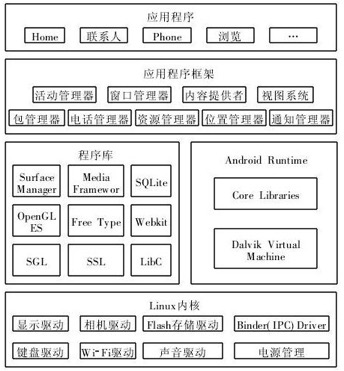
\includegraphics[width=0.8\textwidth]{figure/android}
    \caption{Android系统架构图}
    \label{fg:android}        
\end{figure}
    

参照图\ref{fg:android} ,由上而下对组成系统各部分的主要组件作以下描述。
\begin{enumerate}
    \item Linux内核 

    Android基于Linux 2.6内核,但并非完全照搬内核,而是对内核作了部分增删和修改,在Linux 2.6内核的基础上,Android核心系统实现了安全性、内存管理、进程管理、网络协议栈和驱动模型等功能,Linux内核也同时作为硬件和软件栈之间的抽象层。
    
    硬件驱动程序:完成与各种硬件的通信,Linux内核提供了大部分设备的驱动程序,如显示屏,摄像头,内存,键盘,无线网络,音频设备,电源等组件。 

系统内存管理:对所有可用的内存进行统一编码管理,定义一整套内存定位,使用与回收的策略。 

系统进程管理:内核管理进程的创建与销毁,管理进程间的通信,以及采取必要的措施避免死锁等内容。 

网络管理系统:无线网络设备工作原理,内核掌控如何读取网络设备中的缓存数据。 
    \item 程序库

程序库是指可供使用的各种标准程序、子程序、文件以及它们的目录等信息的有序集合,Android包含一些C/C++库,Android系统中不同的组件通过应用程序框架可以使用这些库,以下是一些核心库: 

    Surface Manager:管理显示子系统,并且为多个应用程序提供2D和3D图层的无缝融合。

    Media Framework:基于OpenCORE的多媒体框架,支持多种常用的音频、视频格式文件的回放和录制,同时支持静态图像文件。 

    SQLite:一个对于所有应用程序可用,功能强劲的轻型关系型数据库引擎。 

    OpenGL ES:3D图形库,用于3D图形渲染,该库可以使用3D硬件加速。 

    FreeType:位图(Bitmap)和矢量(Vector)字体显示。 

    WebKit:支持Android浏览器和一个可嵌入的Web视图。 

    SGL:2D图形库,用于2D图形渲染。 

    LibC:一个从BSD继承的标准C系统函数库,它是专门为基于嵌入式Linux设备定制的。 

    
    \item Android运行库(Android Runtime)

    Android运行库包括两部分:一是核心库,二是自身的虚拟机。 

    核心库提供Java编程语言核心库的大多数功能。Dalvik虚拟机是Google专为Android开发的,比SunJava虚拟机的效率更高,功能也更为复杂,以更好的支撑Android平台,并拥有独立的版权。每一个Android应用程序都在自己的进程中运行,都拥有一个独立的Dalvik虚拟机实例, Dalvik虚拟机执行.dex的可执行文件,该格式文件针对小内存的使用进行了优化,同时虚拟机是基于寄存器实现的,所有的类由Java编译器编译,然后通过SDK中的相应工具转化成.dex格式,最后由虚拟机执行。
    \item 应用程序框架

 应用程序框架是指定义了一个应用程序运行所必须的全部功能组件,开发者也可以访问核心应用程序所使用的API框架。该应用程序的架构设计简化了组件的重用;任何一个应用程序都可以发布它的功能块,并且任何其他的应用程序都可以使用其所发布的功能块(应该遵循框架的安全性限制)。同样,该应用程序的重用机制也使用户可以方便地替换程序组件。
    \item 应用程序 

    Android系统发布时,会同一系列核心应用程序和常用程序一起发布,如常用的手机功能程序,包括语音电话、通讯录、短信收发、照相、话机设置等;数据应用程序,包括邮件工具,日程表,浏览器,地图导航等,以及Android Market上的各种应用程序;所有的应用程序都是使用Java语言编写。 
    
\end{enumerate}


\section{NDK简介}

   NDK 即 Native Development Kit,NDK 是 Google 发布的一系列开发工具集合,这个工具可以帮助 Android 应用程序开发者编译来自 C/C++语言编写的源代码,然后嵌入到他们自己的应用包中,供应用程序调用。Android 的虚拟机在应用程序的源代码中通过JNI调用方法实现本地代码。在内核层面,这意味着你的应用程序源代码可以用关键字native方式声明一个或多个方法,用于指出这些方法是通过本地代码方式实现的;另外你必须提供一个本地共享库包含上述用关键字native声明的方法的具体实现代码。这个库是要被打包到应用程序的apk文件中,而且库的命名也要跟Unix的规则,即lib<something>.so,将包含一个标准的JNI入口点。

   NDK 集成了交叉编译器,并提供了相应的MK文件隔离CPU、平台、ABI 等差异。MK文件相当于配置文件,开发人员在MK 文件中设置一些参数、欲编译的文件及编译特性的要求等,这样编译器就可以根据 MK 文件创建出动态库 so 文件。为了更好的与C/C++开发相结合,也在不断完善开发中,目前 NDK 提供了一些稳定 API 头文件声明,但是在功能上还是相当有限,包括 C 标准库(libc)、标准数学库(libm)、压缩库(libz)、Log库(liblog)。随着版本的不断升级,功能将越来越强大。

\section{OpenCV简介}

OpenCV是近年来推出的开源、免费的计算机视觉库,利用其所包含的函数可以很方便地实现数字图像和视频处理\cite{秦小文2011基于} 。同时利用面向对象的VC++ 6.0编程工具,用C++语言进行程序编写,大大提高了计算机的运行速度。本文首先阐述了OpenCV的特点以及结构,然后以平滑处理、图像形态学为例介绍了OpenCV在数字图像处理中的典型应用。OpenCV算法库为VC++编程处理数字图像提供了很大的方便,其必将成为图像视频处理领域的强有力的工具。

利用OpenCV视觉库,科研开发人员只需添加自己的编写程序,直接调用OpenCV中的函数即可实现,这样不仅降低了开发程序的难度,而且缩短了相关程序的开发周期。

\section{常见图像处理方法}
    在手势识别中有很多常用的图像操作,例如图像的剪切、图像的缩放、图像的旋转以及图像的亮度调整\cite{何阳清2004基于几何特征的手势识别算法研究} 。我们以\emph{Pixe1Array[x,y]}来表示原有图像的二维像素矩阵,原有图像的高度用H来表示,原有图像的宽度用\emph{W}来表示,用\emph{PjxelArrayNew[x,y]}来表示结果图像的二维像素矩阵,结果图像的高度为\emph{HNew},宽度为\emph{WNew}。

\subsection{图像的剪切}

    图像的剪切操作的函数原型为\emph{void CImage::eliplmage(eReet\&reet)},需
要输入的参数为要剪切的图像的具体的位置,即要剪切图像左上角的位置和右下角的位置。

假定要剪切图像左上角位置为\emph{(left,top)},右下角的位置\emph{(right,bottom)},那我们只需要调整图像的宽度为\emph{(righi-left)},调整图像的高度\emph{(bottom-top)},从图像的二维数组中提取左上角到右下角之间的数据。剪切后图像的数据可以表示为:
$$
    PixelArray[x,y] ,\ \ \ left\leq x \leq right \ \ \wedge\ \  top \leq y \leq bottom
$$
\subsection{图像的缩放}

    图像的缩放操作的函数原型为\emph{void CImage::CollapseOrExpandlmage(double dbRatioX,double dbRatioY)}\cite{殷涛2004基于几何矩的手势识别算法}。输入的参数为图像水平方向需要缩放的尺度以及图像垂直方向需要缩放的尺度。

假定水平方向缩放的比例为\emph{a},垂直方向缩放的比例为\emph{b},那么,缩放后图像的高度为\emph{bH},缩放后图像的宽度为\emph{aW},对于原有图像的任一点\emph{PixelArray[x,y]},在缩放后对应的像素为:
$$
    PixelArray[i,j] ,\ \ \ ax\leq i \leq a(x+1) \ \ \wedge\ \  by \leq j \leq b(y+1)
$$


    令\emph{CountArray[i,j]}为结果图像中点\emph{(i,j)}对应原有图像像素的计数,那么每次有点映射到点\emph{(i,j)}的像素时,将结果图像中点\emph{(i,j)}的像素值加上该原有图像点\emph{(x,y)}的像素值,并将\emph{CountArray[i,j]}加1。
$$
    PixelArrayNew[i,j]=PixelArrayNew[i,j]+PixelArray[x,y]
$$
$$
    CountArray[i,j]=CountArray[i,j]+1
$$

由于经缩放后,结果图像中的某一点的像素可能对应原有图像中的多个像素,所以对于这种情况需要对该点的像素求取平均值:
$$
    PixelArrayNew[i,j]=\frac{PixelArrayNew[i,j]}{CountArray[i,j]} %PixelArrayNew[i,j]/CountArray[i,j]
$$


    图像缩放操作可以用一个简单的示意图(图\ref{fg:ss})来表示:
    
\begin{figure}[htb]
    \centering
    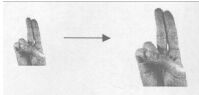
\includegraphics[width=0.5\textwidth]{figure/suofang}
    \caption{缩放示意图}
    \label{fg:ss}
\end{figure}

\subsection{图像的旋转}

    图像的旋转在所有的通用操作中是最复杂的,它的函数原型为\emph{void CImage::Rotatelmage(double dbAngle)}。从中可以看出,传入的参数是需要旋转的角度,该角度以弧度值来表示,正数表示的是逆时针方向旋转,负数表示的是顺时针方向旋转。

旋转操作的示意图如图\ref{fg:roat}所示(逆时针旋转\emph{Q}度):
\begin{figure}[htb]
    \centering
    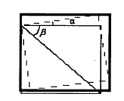
\includegraphics[width=0.5\textwidth]{figure/roat}
    \caption{旋转示意图}
    \label{fg:roat}
\end{figure}
      

图中细黑色的表示原来图像的范围,粗黑色的为旋转后图像的范围,虚线的为原来图像经旋转后在结果图像中的位置。

旋转操作首先需要判断该角度属于哪一个象限,不同的象限所使用的变换公式是不同的。假定输入的旋转角度为$\theta $,令$\theta_1 $为$\theta$经变换后在$[0,2\pi ]$之间的角度,令$\alpha $ 为$\theta $经变换后在$[0,\pi /2 ]$之间的角度,其中:
$$
\alpha =\left\{ 
    \begin{aligned}
       & \theta_1 &0 \leq \theta_1 \leq \pi /2 \\
       & \theta_1 -\pi &\pi /2 < \theta_1 \leq \pi\\
       & \theta_1 -\pi &\pi < \theta_1 \leq 3\pi /2\\
       & \theta_1 -3\pi /2 \ \ \ &3\pi /2 <\theta_1 \leq 2\pi 
    \end{aligned}
\right.
$$
令
$$
\begin{aligned}
NW&=Wcos\alpha +Hsin\alpha \\
NH&=Wsin\alpha +Hcos\alpha 
\end{aligned}
$$
对于原图像中的点$(x,y)$,在新图像中对应的坐标为$(x',y')$,那么
\begin{enumerate}
    \item $\theta $在第一象限时$$HNew=NH,WNew=NW$$
    $$
    \begin{aligned}
      x'&=xcos\alpha +ysin\alpha\\
      y'&=(W-x-1)sin\alpha +ycos\alpha
    \end{aligned}
    $$
    \item $\theta $在第二象限时$$HNew=NW,WNew=NH$$
    $$
    \begin{aligned}
      x'&=(W-x-1)sin\alpha +ycos\alpha\\
      y'&=NW-1-xcos\alpha -ysin\alpha
    \end{aligned}
    $$
    \item $\theta $在第三象限时$$HNew=NH,WNew=NW$$
     $$
    \begin{aligned}
      x'&=NW-1-xcos\alpha -ysin\alpha\\
      y'&=NH-1-(W-x-1)sin\alpha -ycos\alpha
    \end{aligned}
    $$
    \item $\theta $在第四象限时$$HNew=NH,WNew=NW$$
     $$
    \begin{aligned}
      x'&=NH-1-(W-x-1)sin\alpha -ycos\alpha\\
      y'&=xcos\alpha +ysin\alpha
    \end{aligned}
    $$
\end{enumerate}
这样在任意的旋转角度下,原图像中的每一点都可以对应到新图像中的某一点中,考虑到经过旋转后在新图像中对应原图像部分的内部可能存在某些点在原图像中不存在对应点,所以需要对这些点作平滑处理,使图像达到连续的效果。
假定对于图像中的任一点$PixelArrayNew[x,y]$,如满足条件:
$$
\begin{aligned}
    PixelArrayNew[x,y] \ \ &\wedge\ \  \\
    PixelArrayNew[x-1,y]\neq 0 \ \ &\wedge\ \ PixelArrayNew[x+1,y]\neq 0 \\
    PixelArrayNew[x,y-1]\neq 0\ \ &\wedge\ \ PixelArrayNew[x,y+1]\neq 0
\end{aligned}
$$
则
$$
\begin{aligned}
     PixelArrayNew[x,y]&=\\
    &(PixelArrayNew[x-1,y]+PixelArrayNew[x+1,y]\\
    &+PixelArrayNew[x,y-1]+PixelArrayNew[x,y+1])/4
\end{aligned}  
$$
\ifx\allfiles\undefined
%\bibliographystyle{unsrt}
\bibliography{main}
\end{document}
\fi